

%proof of concept 
%chalanges 
%requirments of stream processing %https://www.slideshare.net/arunkejariwal/modern-realtime-streaming-architec%tures?qid=f9d8532f-94be-47ee-bdf1-045826ba283e&v=&b=&from_search=1


\frame
{
	\frametitle{Motivation}
	\framesubtitle{A New Era: Big event Data streams}
		\begin{center}
		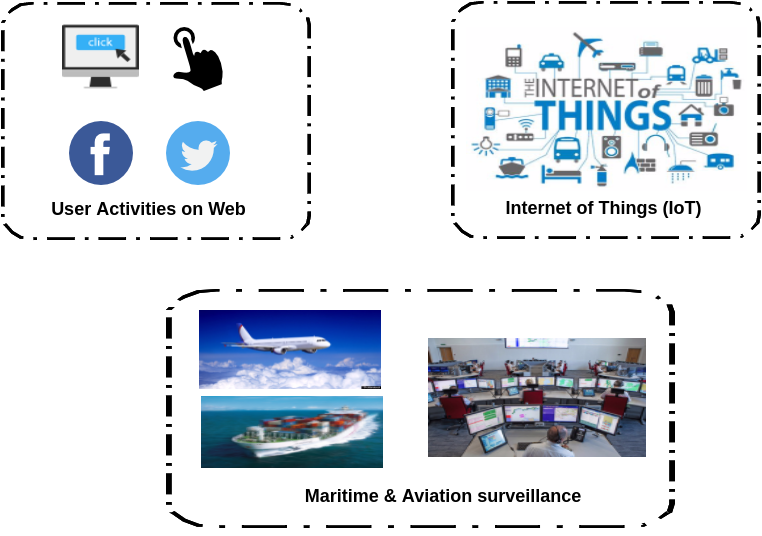
\includegraphics[scale=.36]{figures/motiv.png}\\
		.
	\end{center}
}


\frame
{
\frametitle{Motivation}
\framesubtitle{A New Era: Big event Data streams}
\begin{center}
	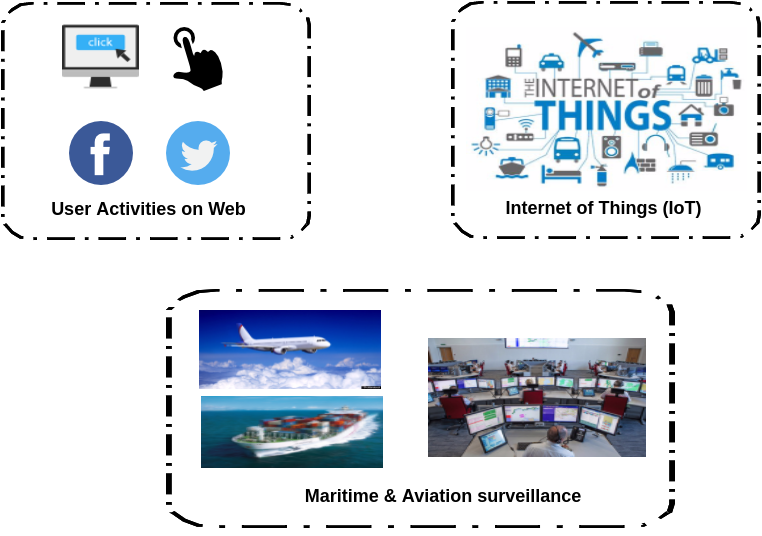
\includegraphics[scale=.3]{figures/motiv.png}\\
	.
\end{center}
	

	\begin{itemize}[]
		
		\item<1-> Common Goal: recognition and prediction full matches of complex event patterns in real-time.
%		\item<1-> improve operational efficiency.
%		\item<1 -> enable proactive decision making.
		
	\end{itemize}
}


\frame
{
	\frametitle{Problem Formulation}
	
	\begin{itemize}[]
		\item<only@1>Given a set of $k$ real-time streams of events $S = \{ s_1,s_2, ..., s_k\}$.
		
		\item<only@1> Each stream  $s_i=\langle e_1,e_3,...,e_t,...\rangle$  is a time-ordered infinite sequence of events.
		
		\item<only@1> Each event is defined as a tuple of attributes $e_i = (id,type,\tau,a_1,a_2,\ldots,a_n)$, where $type\ \in  \Sigma$ (i.e., event types), $\tau\in\R$, and  $id\in\N$ . 
		\item<only@1> A user-defined pattern $\mathcal{P}$ is given in the form of a regular expression over a set of event types. $\Sigma$ ($\mathcal{P} := E\ |\ \mathcal{P}_{1} ; \mathcal{P}_{2}\ | \mathcal{P}_{1} \vee \mathcal{P}_{2}\ |\ \mathcal{P}_{1}^{*}$,  $E \in \Sigma$).
		
		
		\item<2->The main objective is to predict the pattern $\mathcal{P}$ completion with certain probability in the future over each stream $s_i$ given the current time event $e_t$. 
		
		\item<3-> (\textbf{Pattern Prediction over Multiple Event Streams})
	\end{itemize}
}

\begin{frame}[fragile]

	\frametitle{An Illustrative Application Domain:}
    \framesubtitle{Maritime Surveillance}
	\begin{itemize}
%		\item<only@1> Process  emitted from moving vessels or derived critical points of vessel trajectories as input event streams.
		\item<only@1> Event tuple (i.e., critical points) derived from raw Automatic Identification System (AIS) messages of moving vessels e.g., 
		\begin{minted}{json}
	{
	"timestamp":1443651492000,
	"id":"228133000",
	"annotation":"change_in_heading",
	"latitude":48.117775,
	"longitude":-4.4205885,
	"distance":323.406,
	"heading":264.27
	"speed":18.48,
	}
	\end{minted}
	
		\item<only@1> Example patterns such as:\\
 	   $\mathcal{P}_1=Sailing$ or\\ 
 	   $\mathcal{P}_2=changeInHeading; gapStart; gapEnd; changeInHeading$
	\end{itemize}
\end{frame}

